\chapter{Marco teórico y Antecedentes }
\hrule \bigskip \vspace*{1cm}
%------------------------------------------------------------------------

\section{Desambiguación del sentido de las palabras (WSD)}
En general, la desambiguación del sentido de las palabras es el problema de seleccionar un sentido de un conjunto de posibilidades predefinidas para una palabra dada en un texto o discurso. 
En los últimos años se han incrementado las investigaciones para crear métodos de WSD. A continuación, se describe la clasificación para métodos de WSD de acuerdo a los recursos que utilizan (figura 2.1).

  \begin{figure}[h!]
	  \begin{center}
    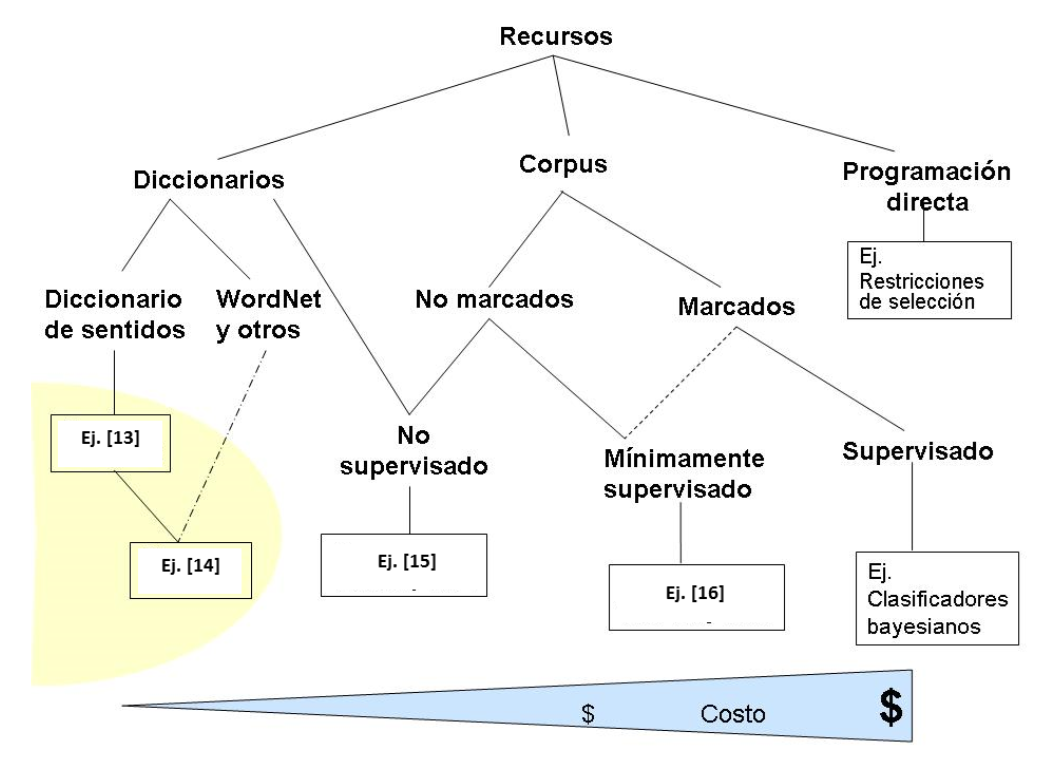
\includegraphics[angle=0, width=10cm]{Graficos/desambiguacion_WSD}
	  \caption{Clasificación de los métodos para WSD de acuerdo a los recursos que utilizan [1].}
    \end{center}
	\end{figure}

\section{Clasificación de sistemas en WSD}
\subsection{Métodos basados en conocimiento}
En esta categoría encontramos diferentes algoritmos para la etiquetación automática de sentidos. Normalmente, el rendimiento de estos métodos basados en conocimiento, es menor en comparación con los métodos basados en corpus. Pero con la salvedad de que los métodos basados en conocimiento tienen una amplia cobertura ya que pueden aplicarse a cualquier tipo de texto en comparación con los basados en corpus que sólo se pueden aplicar a aquellas palabras de las que se dispone de corpus anotados. A continuación, vamos a enumerar diferentes técnicas utilizadas por los métodos basados en conocimiento, aplicables sobre cualquier base de conocimiento léxica que defina sentidos de palabras y relaciones entre ellas. La base de conocimiento léxica más utilizada es WordNet (Miller (1995)). Vamos a describir 4 tipos diferentes de métodos basados en conocimiento:

\begin{itemize}
  \item Algoritmo de Lesk
  \item Similitud semántica
  \item Preferencias de selección
  \item Métodos Heurísticos
\end{itemize}

\subsubsection{Algoritmo de Lesk}
El algoritmo de Lesk [2] es uno de los primeros algoritmos exitosos usados en la desambiguación de sentidos de palabras. Este algoritmo se basa en dos puntos principales: un algoritmo de optimización para WSD y una medida de similitud para las definiciones de los sentidos.
El primer punto es acerca de desambiguar palabras considerando la coherencia global del texto, esto es, encontrar la combinación de los sentidos que maximice la relación total entre los sentidos de todas las palabras. 
Por ejemplo, para la oración \textit{My father deposits his money in a bank account} y considerando a lo más tres sentidos (véase tabla 1), para cada palabra, la figura 2 muestra la representación gráfica del algoritmo original de Lesk.

  \begin{figure}[h!]
    \begin{center}
    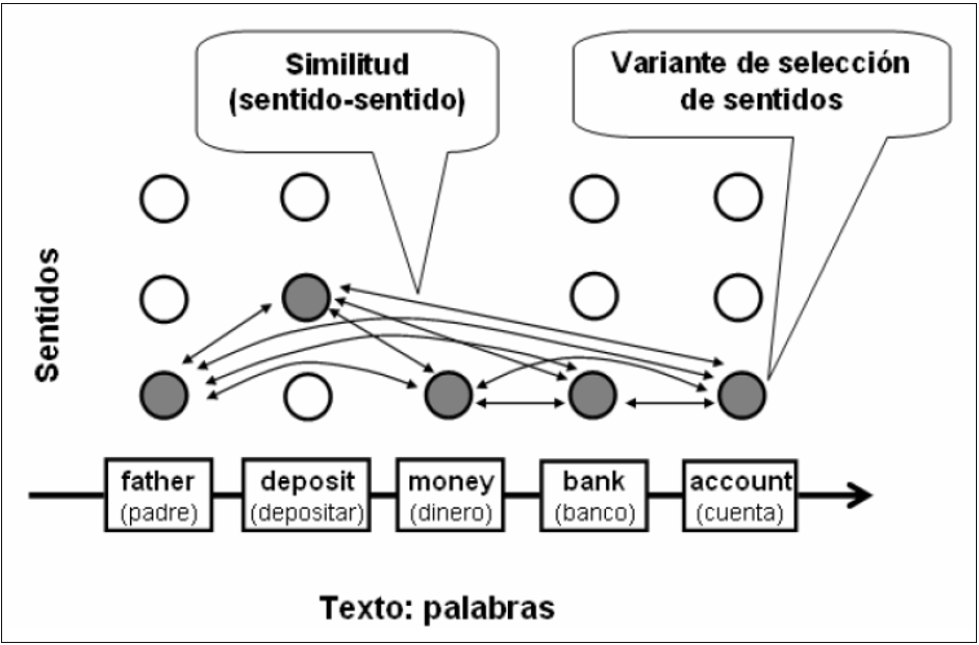
\includegraphics[angle=0, width=10cm]{Graficos/algoritmo_lesk}
    \caption{Representación gráfica del algoritmo original de Lesk [1]}
    \end{center}
  \end{figure}

  \begin{table}[t]
    \centering
      \begin{tabular}{|m{2cm}|m{10cm}|}
      \hline
      % after \\: \hline or \cline{col1-col2} \cline{col3-col4} ...
      Palabra & Sentidos\\
      \hline
      \hline
      Father & 1: a male parent (also used as a term of address to your father); "his father was born in Atlanta". 
      2: `Father' is a term of address for priests in some churches (especially the Roman Catholic Church or the Orthodox Catholic Church); “`Padre' is frequently used in the military”. 
      3: a person who holds an important or distinguished position in some organization; "the tennis fathers ruled in her favor"; "the city fathers endorsed the proposal".\\
      \hline
      Deposit & 1: fix, force, or implant; "lodge a bullet in the table". 
      2: put into a bank account; "She deposits her paycheck every month". 
      3: put (something somewhere) firmly; "She posited her hand on his shoulder"; "deposit the suitcase on the bench"; "fix your eyes on this spot".\\
      \hline
      Money & 1: the official currency issued by a government or national bank; "he changed his money into francs".  \\
      \hline
      Bank & 1: a financial institution that accepts deposits and channels the money into lending activities; "he cashed a check at the bank"; "that bank holds the mortgage on my home". 
      2: sloping land (especially the slope beside a body of water); "they pulled the canoe up on the bank"; "he sat on the bank of the river and watched the currents". 
      3: a supply or stock held in reserve for future use (especially in emergencies) \\
      \hline
      Account& 1: a formal contractual relationship established to provide for regular banking or brokerage or business services; "he asked to see the executive who handled his account". 
      2: the act of informing by verbal report; "he heard reports that they were causing trouble"; "by all accounts they were a happy couple". 
      3: a record or narrative description of past events; "a history of France"; "he gave an inaccurate account of the plot to kill the president"; "the story of exposure to lead".\\
      \hline
    \end{tabular}
    \caption{Sentidos de las palabras (máximo tres) obtenidas de WordNet para la oración \textit{“My father deposits his money in a bank account”}.[1]
    }\label{tab:demo}
  \end{table}

En el segundo punto, relacionado con la medida de similitud, Lesk sugiere usar el traslape entre las definiciones de los sentidos, es decir, contar el número de palabras que tienen en común. 
Como ejemplo, para la oración, \textit{“My father deposits his money in the bank ac-count”} para medir la relación de las definiciones de los sentidos para la palabra \textit{“de-posit”} y \textit{“bank”} como Lesk lo propuso, es necesario contar las palabras en común en todas las definiciones. En este caso, comparando principalmente las tres definiciones de \textit{“deposit”} contra las tres definiciones de “bank”. La relación entre los valores se muestra en la tabla 2.

\begin{table}[t]
  \centering
    \begin{tabular}{|m{4cm}|m{4cm}|m{4cm}|}
      \hline
      Sentido elegido para \textit{deposit} & Sentido elegido para \textit{bank} & Valor de relación (traslape de palabras)\\
      \hline
      1 & 1 & 0 \\
      \hline
      1 & 2 & 0 \\
      \hline
      1 & 3 & 0 \\
      \hline
      2 & 1 & 2 \\
      \hline
      2 & 2 & 1 \\
      \hline
      2 & 3 & 0 \\
      \hline
      3 & 1 & 1 \\
      \hline
      3 & 2 & 0 \\
      \hline
      3 & 3 & 0 \\
      \hline
     \end{tabular}
   \caption{Sentidos de las palabras (máximo tres) obtenidas de WordNet para la oración \textit{“My father deposits his money in a bank account”}.[1]
  }\label{tab:demo2}
\end{table}

Este algoritmo tiene dos limitaciones, por un lado, la limitación principal de la medida de similitud propuesta por Lesk, es que las glosas del diccionario, regularmente, son muy cortas y no incluyen el vocabulario suficiente para identificar los sentidos relacionados [3]. 
Por otro lado, mientras más palabras tenga el texto, y más sentidos por cada palabra, mayor será el número de combinaciones de sentidos, haciéndolo prácticamente prohibitivo para una búsqueda exhaustiva que garantice encontrar el óptimo global exacto. Por ejemplo, para una oración de 16 palabras de contenido, donde cada palabra contiene siete sentidos (números cercanos a los observados en el corpus de SemCor), existen 716 posibles combinaciones a escoger, de las cuales una será seleccionada. 
Debido a estas dos limitaciones, diferentes modificaciones al algoritmo original han sido propuestas para mejorar los resultados en la desambiguación de sentidos de palabras, las cuales se describen en la siguiente sección.

\begin{itemize}
  \item \textbf{Lesk simple o Lesk simplificado} \\
    Para reducir el espacio de búsqueda del algoritmo original de Lesk, Kilgarriff y Rosenzweig [4] propusieron una variación del algoritmo original de Lesk, conocido como algoritmo de \textbf{Lesk simplificado o Lesk simple}, donde los sentidos de las pala-bras en el texto son determinados uno a uno encontrando el mayor traslape entre los sentidos de las definiciones de cada palabra con el contexto actual, véase la figura 3. En lugar de buscar asignar, simultáneamente, el significado de todas las palabras en un texto dado, este enfoque determina el sentido de las palabras uno a uno, por lo que se evita la explosión combinatoria de sentidos.
  
    \begin{figure}[h!]
      \begin{center}
      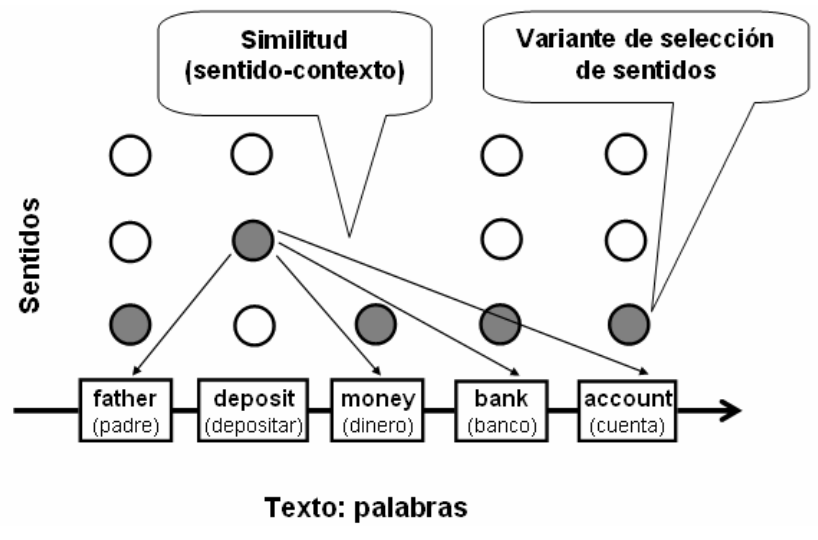
\includegraphics[angle=0, width=10cm]{Graficos/lesk_simple}
      \caption{Representación gráfica del algoritmo de Lesk simplificado [1]}
      \end{center}
    \end{figure}
    
    \item \textbf{Templado simulado (Simulated Annealing)} \\
    El método de templado simulado es una técnica para la resolución de problemas de optimización combinatoria a gran escala. El nombre de este algoritmo es una analogía del proceso metalúrgico en el cuál, el metal se enfría y se templa. La característica de este fenómeno es que en el enfriamiento lento alcanza una composición uniforme y un estado de energía mínimo, sin embargo, cuando el proceso de enfriamiento es rápido, el metal alcanza un estado amorfo y con un estado alto de energía. En templado simulado la variable \textbf{T} corresponde a la temperatura que decrece lentamente hasta encontrar el estado mínimo. 
    El proceso requiere una función \textbf{E}, la cual representa el estado de energía de cada configuración del sistema. Es esta función la que se intenta minimizar. A grandes rasgos el algoritmo funciona de la siguiente manera: se selecciona un punto inicial y además se escoge otra configuración de manera aleatoria, se calcula para ambas con-figuraciones su valor \textbf{E}, si el nuevo valor es menor que el seleccionado como punto inicial, entonces el inicial es remplazado por la nueva configuración. Una característica esencial del templado simulado es que, existe el caso en el que la nueva configuración es mayor a la configuración obtenida anteriormente, y la nueva es seleccionada. Esta decisión es tomada de manera probabilística y permite salir de algún mínimo local. Una vez que el método mantenga la misma configuración por un determinado tiempo, dicha configuración es escogida como la solución. 
    Cowie et al. [5], basándose en el algoritmo de Lesk, utilizó este método para desambiguación de sentidos de palabras de la siguiente forma: 
    \begin{enumerate}
      \item El algoritmo define una función \textbf{E} para la combinación de sentidos de palabras en un texto dado. 
      \item Se calcula \textbf{E} para la configuración inicial \textbf{C}, donde \textbf{C} es el sentido más frecuente para cada palabra.
      \item Para cada iteración, se escoge aleatoriamente otra configuración conocida como \textbf{C’}, y se calcula su valor de \textbf{E}. Si el valor de \textbf{E} para \textbf{C’} es menor que el de \textbf{C} entonces se elige \textbf{C’} como configuración inicial.
      \item  La rutina termina cuando la configuración de sentidos no ha cambiado en un tiempo determinado.
    \end{enumerate}
  
  \item Medida de Lesk Adaptada
    Lesk propuso medir la similitud entre sentidos contando el traslape de palabras. La limitación principal de esta técnica es que las glosas del diccionario, por lo general, son muy breves, de tal manera que no incluyen suficiente vocabulario para identificar los sentidos relacionados. En [6] se sugiere una adaptación del algoritmo basado en WordNet. Esta adaptación consiste en tomar en cuenta las glosas de los vecinos de la palabra a desambiguar, explotando los conceptos jerárquicos de WordNet, de tal ma-nera que las glosas de los vecinos son expandidas incluyendo a su vez las glosas de las palabras con las cuales se encuentran relacionadas mediante las diversas jerarquías que presenta WordNet. Así mismo, sugieren una variación en la manera de asignar el puntaje a una glosa, de tal manera que si “n” palabras consecutivas son iguales en ambas glosas, estas deberán de tener mayor puntaje que aquel caso en el que sólo coincide una sola palabra en ambas glosas. 
    Supongamos que \textit{bark} (ladrido o corteza) es la palabra que se desea desambiguar y sus vecinos son textit{dog} (perro) y textit{tail} (cola). El algoritmo original de Lesk verifica las coincidencias en las glosas de los sentidos de textit{dog} con las glosas de textit{bark}. Luego verifica las coincidencias en las glosas de textit{bark} y textit{tail}. El sentido de textit{bark} con el máximo número de coincidencias es seleccionado. La adaptación del algoritmo de Lesk consi-dera estas mismas coincidencias y añade además las glosas de los sentidos de los conceptos que se encuentran relacionados semántica o léxicamente a textit{dog}, textit{bark} y textit{tail}, de acuerdo a las jerarquías de WordNet.
\end{itemize}

\subsubsection{Similitud semántica}
\subsubsection{Preferencias de selección}
\subsubsection{Métodos Heurísticos}
\subsection{Métodos basados en corpus no supervisados}
\subsection{Métodos basados en corpus supervisados}
\subsection{Métodos híbridos}
%La forma como colocar un algoritmo es mediante el
%\verb"\usepackage{algorithmic}" y \verb"{algorithm}" este imprime de
%la siguiente forma:

\bigskip
\begin{algorithm}
\caption{Mapeamiento}\label{mapeadoEVA} processo\_ID(Identificación de flags)\\
Require: Lista de ${1\ldots N}$ que contenga los ID de las clases
correspondientes(provenientes del $FM$).
\begin{algorithmic} [1]
\STATE Generar \emph{lista} a partir de pares correspondientes según
$FM$ \WHILE {SchemaB contenga alguna clase}
\IF{valorASIG(\emph{claseB}) $\geq$ parametro \verb"VAL"}\STATE
\emph{claseB} $\Longleftarrow$ siguiente clase de SchemaB \STATE
\emph{lista} $\Longleftarrow$ agregar los términos de \emph{claseB}
y su correspondiente \emph{claseA} \STATE valor
(\emph{lista$(A_{i},B_{j})$})=\verb"POS"=$1$ \ENDIF \ENDWHILE
\end{algorithmic}
\end{algorithm}

NOTA: Este package no viene incluido por default en el \LaTeX ni con
esta plantilla, pero si es de mucha utilidad, esta disponible en
internet así como muchas otras. Si desean incluir un nuevo
\verb"\usepackage{Nombre_Package}", solo deben agregarla en el
archivo \verb"unsa.cls" en una linea y ya estará disponible.
